\documentclass{../../tex_template/asaproc}
\usepackage{graphicx} % \includegraphics
\usepackage{float}    % To keep figures in right place. 
                      % Usage: \being{figure}[H] \includegraphics{tmp.pdf} \end{figure}
\usepackage{subfig}   % \subfloat
\usepackage{amsmath}  % bmatrix, pmatrix, etc
\usepackage{bm}
\newcommand{\p}[1]{\left(#1\right)}
\newcommand{\bk}[1]{\left[#1\right]}
\newcommand{\bc}[1]{ \left\{#1\right\} }
\newcommand{\abs}[1]{ \left|#1\right| }
\newcommand{\norm}[1]{ \left|\left|#1\right|\right| }
\newcommand{\E}{ \text{E} }
\newcommand{\N}{ \mathcal N }
\newcommand{\ds}{ \displaystyle }

%\usepackage{times}
%If you have times installed on your system, please
%uncomment the line above

%For figures and tables to stretch across two columns
%use \begin{figure*} \end{figure*} and
%\begin{table*}\end{table*}
% please place figures & tables as close as possible
% to text references

\newcommand{\be}{\begin{equation}}
\newcommand{\ee}{\end{equation}}
\newcommand{\y}{\bm y}
\newcommand{\X}{\bm X}

\title{FYE--- Ozone}

%input all authors' names
\author{
  Arthur Lui$^1$\\
  University California -- Santa Cruz$^1$\\
}

%input affiliations
%{USDA Forest Service Forest Products Laboratory}

\begin{document}
\maketitle
\begin{abstract}
ABSTRACT GOES HERE!!!
\begin{keywords}
KEYWORDS GO HERE!!!
Bayesian Regression, Ozone, temperature, wind speed, radiation
\end{keywords}
\end{abstract}

\section{Introduction}
INTRODUCTION GOES HERE!!!
High ozone-level-exposures are known to be associated with the development of respiratory
and other diseases.


\subsection{Exploratory Analysis}
Plotted in Figure \ref{fig:pairs} is a scatter plot matrix of the distribution of 
Ozone concentration (ppb), radiation (0 for low, 1 for moderate to high levels),
temperature (F$^\circ$), and wind speed (mph). Along the diagonal are the univariate
histograms. For each of the mentioned variables. Worthy of mention is the Ozone
concentration, which distribution is heavy tailed.
\begin{figure}[H]
  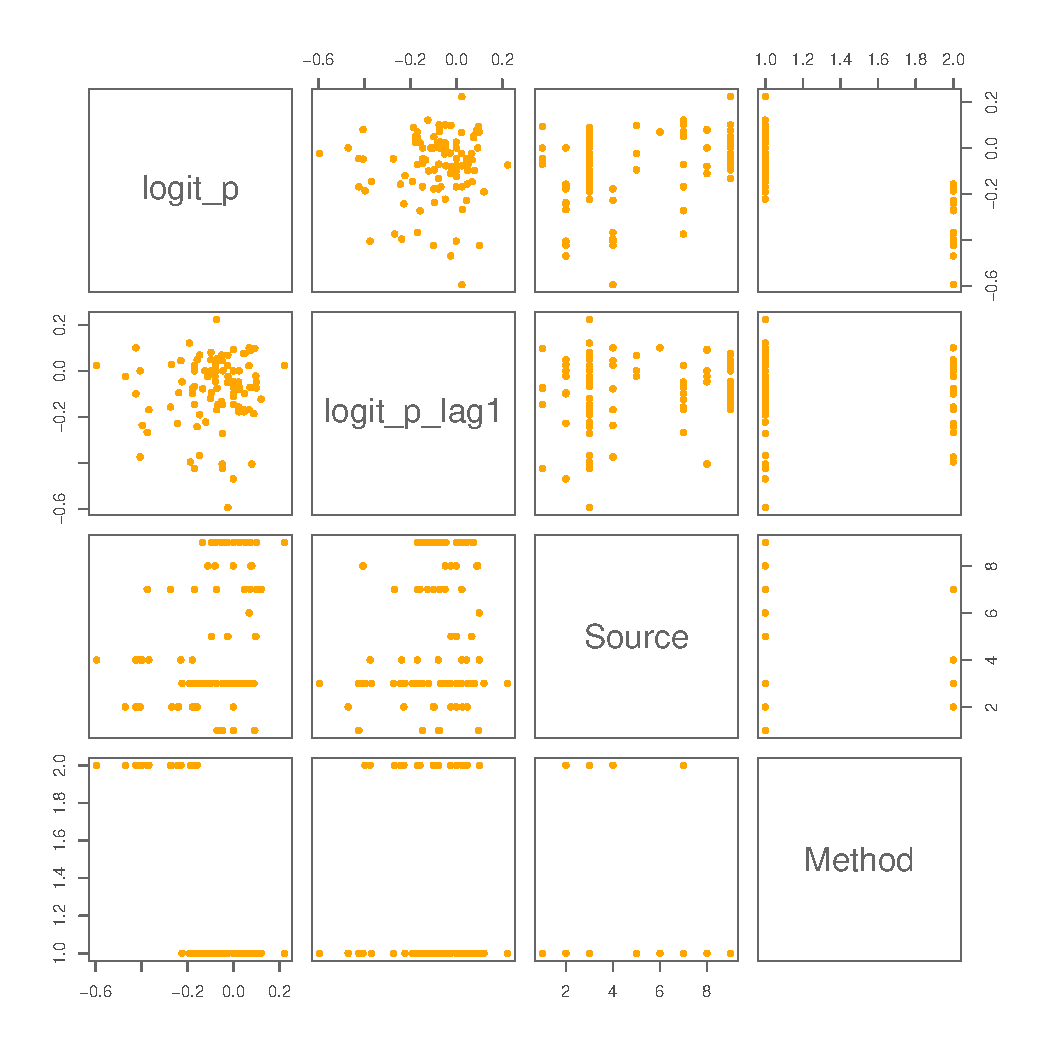
\includegraphics[scale=.5]{figs/pairs.pdf}
  \caption{\small Scatter plot matrix of ... }
  \label{fig:pairs}
\end{figure}
For modeling purposes, transforming Ozone concentration to log Ozone
concentration may be beneficial, so it is done.  The resulting scatter plot
matrix is shown in Figure \ref{fig:logpairs}.
\begin{figure}[H]
  \includegraphics[scale=.5]{figs/log_ozone_pairs.pdf}
  \caption{\small Scatter plot matrix of ... }
  \label{fig:logpairs}
\end{figure}
Radiation level is a binary variable with approximately two thirds of the
observations being low; the remaining being moderate to high.  Temperature and
wind speed have roughly symmetric distributions. Relative to the other pairs of
variables, Ozone and temperature have a large correlation of .745.  All other
pairs of variables have at moderate correlation with the exception of radiation
level and wind speed. Moreover, temperature exhibits a linear trend between
all other variables.

Given this preliminary analysis, a good candidate linear model is that with
response variable $\y$ being the log Ozone concentration, and covariates being
radiation level, temperature, and wind speed. This is a good candidate model
because the Ozone concentration is linear with the covariates and the 
covariates are not strongly correlated. (Independence among covariates avoids
the problem of inflated variances of the covariates in a model with
multicollinearity.)

\section{Methods}
METHODS GO HERE!!!

\section{Analysis}
ANALYSIS GOES HERE!!!
\begin{figure}[H]
  \includegraphics[scale=.5]{figs/posts1.pdf}
  \caption{\small Posteriors of ... }
  \label{fig:posts1}
\end{figure}

\begin{figure}[H]
  \includegraphics[scale=.5]{figs/posts2.pdf}
  \caption{\small Posteriors of ... }
  \label{fig:posts2}
\end{figure}

\begin{figure}[H]
  \includegraphics[scale=.5]{figs/obsvsfit.pdf}
  \caption{\small Posteriors of observed vs. fitted. }
  \label{fig:obsvsfit}
\end{figure}

\begin{figure}[H]
  \includegraphics[scale=.5]{figs/rmse.pdf}
  \caption{\small Posteriors of RMSE. The model with radiation has lower RMSE. The probability that the RMSE in the
   model with radiation as a coavariate is lower than that of the model without radiation is 84\%.}
  \label{fig:rmse}
\end{figure}

\begin{figure}[H]
  \includegraphics[scale=.5]{figs/map.pdf}
  \caption{\small Heatmap of ...}
  \label{fig:map}
\end{figure}

\section{Conclusions}
CONCLUSIONS GO HERE!!!

\begin{references}
{\footnotesize
\itemsep=3pt
\item {\em Gelman, A., Carlin, J. B., Stern, H. S., \& Rubin, D. B. (2014). Bayesian data analysis (Vol. 2). Boca Raton, FL, USA: Chapman \& Hall/CRC, 73.}
}

\end{references}
\end{document}

%\begin{figure*}
%  \centering
%  \includegraphics[scale=.55]{figs/mapDat.pdf}
%  \vspace{-7em}
%  \caption{\small Some Caption.}
%  \label{fig:mapDat}
%\end{figure*}

%\begin{figure}[H]
%  \includegraphics[scale=.5]{figs/pairsLogRate.pdf}
%  \caption{\small Hi Motor vehicle theft is not strongly correlated with any other thefts.}
%  \label{fig:logOdds}
%\end{figure}
